\documentclass[useAMS,usenatbib]{mn2e}
\usepackage{graphicx}
\newcommand{\figpath}{./Figs/}

% If your system does not have the AMS fonts version 2.0 installed, then
% remove the useAMS option.
%
% useAMS allows you to obtain upright Greek characters.
% e.g. \umu, \upi etc.  See the section on "Upright Greek characters" in
% this guide for further information.
%
% If you are using AMS 2.0 fonts, bold math letters/symbols are available
% at a larger range of sizes for NFSS release 1 and 2 (using \boldmath or
% preferably \bmath).
%
% The usenatbib command allows the use of Patrick Daly's natbib.sty for
% cross-referencing.
%
% If you wish to typeset the paper in Times font (if you do not have the
% PostScript Type 1 Computer Modern fonts you will need to do this to get
% smoother fonts in a PDF file) then uncomment the next line
% \usepackage{Times}

%%%%% AUTHORS - PLACE YOUR OWN MACROS HERE %%%%%


%%%%%%%%%%%%%%%%%%%%%%%%%%%%%%%%%%%%%%%%%%%%%%%%



\title[Geometrically thin acrretion disk around white dwarfs and quark stars]{Geometrically thin acrretion disk around quark stars}
\author[B. Mishra, B. Vaidya and W. Kluzniak]{B. Mishra$^{1}$\thanks{E-mail:
mbhupe@camk.edu.pl}, W. Klu\'zniak$^{1}$, B. Vaidya$^{2}$\\
$^{1}$Copernicus Astronomical Center, Bartycka 18, Warsaw,00-716, Poland\\
$^{2}$University of Leeds, Leeds LS2 9JT, United Kingdom}
\begin{document}



\date{Accepted *** Received ***}

\pagerange{\pageref{firstpage}--\pageref{lastpage}} \pubyear{2014}

\maketitle

\label{firstpage}

\begin{abstract}
We studied semi-analytically and numerically the geometrically thin and optically thick accretion disk around rapidly rotating quark stars and white dwarfs using potential for Maclaurin spheroid. The main interest is to investigate the inner region of the so called $\alpha$-disk. We found that the change in eccentricity of the compact object influence the spectra emitted from the accretion disk. This can be observational evidence for the existance of the quark stars. Analytical calculations are mainly done in the radiation pressure dominated region of the accretion disk. The numerical work has been carried out to see the time evolution of the accretion disk around quark stars and white dwarfs using the same potential for Maclaurin spheroids. We showed that if the eccentricity of the object is high the matter will diffuse slowly and advect rapidly during its evolution. This gives a clue that how spin up or spin down can change the time evolution of the accretion disk using a very simple Newtonian approach.  

\end{abstract}

\begin{keywords}
Maclaurin spheroids, white dwarfs, quark stars, accretion disk
\end{keywords}

\section{Introduction}

\section{Physical Model}
\subsection{MacLaurian Spheroid}
\begin{itemize}
\item Describe in very brief the basics and how $\Omega$ is obtained
  and re-draw the plot that is in your supervisor paper. 
\end{itemize}
\subsection{Analytical Approach}
\begin{itemize}
\item List all the equations that you have used and what modification
  you have done for e.g., you have used $\Omega$ corresponding to
  MacLaurian spheroid. 
\item Say that formulae depends on M, Mdot, $\alpha$, r and
  eccentricity and give the values of choices made for them. 
  Explicit formulae and quantities shall be discussed in results
  section.
\end{itemize}
\subsection{Numerical Evolution}
\begin{itemize}
\item List formulae and refer the paper that we have been using for
  evolution of Surface density. 
\end{itemize}

\section{Results}
\subsection{Steady state disk}
\begin{figure}
\centering
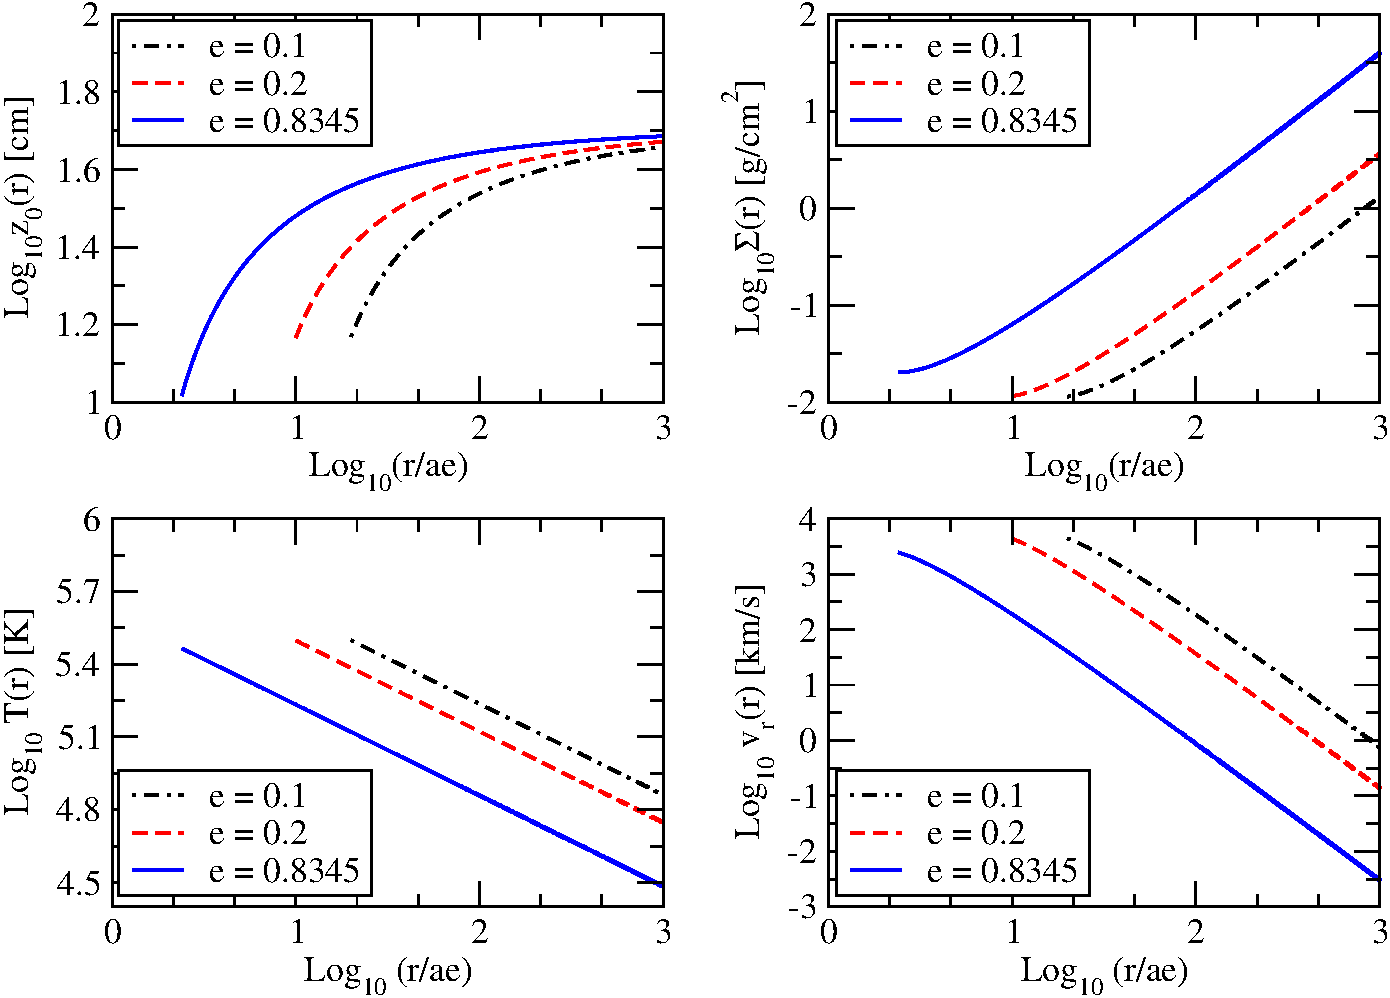
\includegraphics[width=1\columnwidth]{\figpath/multiplot_rho_alpha0001.pdf}
\caption{Multiplot of various quantities obtained from semi-analytical
  work}
\label{fig:steadyplt1}
\end{figure}

\begin{itemize}
\item describe the multi plots (fig~\ref{fig:steadyplt1}) for each quantity : its value, its
  profile and dependence on eccentricity.
\item Make a table which gives quantitive values.  
\end{itemize}


\subsection{Disk thermodynamics and Spectra}
\begin{itemize}
\item Show that values of T obtained above give Prad $>$ Pgas. 
\item Also show that the disk is optically thick.
\item Finally describe the spectra and state its dependence on
  eccentricity. (Explain the reason in discussion).
\end{itemize}
\subsection{Evolution of surface density}
\begin{itemize}
\item Show the plot of evolution of a ring of matter for a particular high
  eccentricity and describe it. Specially the skewed profile for
  higher eccentricity. 
\item Show that at low eccentricity it approaches the $\alpha$-disk
  solution. Here also describe the plot which shows the evolution with
  different eccentricity. 
\end{itemize}

\section{Discussion}
\subsection{Very thin and fast disk}
\begin{itemize}
\item Why few cm sized disk?
\item Is Newtonian gravity responsible for faster disk. 
\item how values change with change in $\alpha$. 
\end{itemize}

\subsection{Dependence of Spectra on eccentricity}
\begin{itemize}
\item Explain the reason for the dependence of spectra on e. 
\item Discuss its consequences in observations.
\end{itemize}

\subsection{Angular Momentum transport in disks}
\begin{itemize}
\item Explain the reason for skewness in sigma plot with high e
  values. Show plots of advection and diffusion. 
\item Also discuss the implication of e on Ang. momentum transport. 
\end{itemize}

\section{Conclusion}
State your conclusions here. 






\label{lastpage}
\end{document}
